\documentclass[12pt, a4paper]{article}
\usepackage[utf8]{inputenc}
\usepackage{ 
    amsmath, amssymb, amsfonts, 
    amsthm, lipsum, 
    physics, mathtools, setspace,
    array, caption, float,
    tikz, tikz-3dplot, multicol,
    stackengine, enumitem
}

\usepackage[hmarginratio=1:1, margin=0.5in, includeheadfoot]{geometry}

\graphicspath{ {./res/} }
\usetikzlibrary{decorations.markings}
\usetikzlibrary{angles, quotes}
\newcommand{\neswarrow}{\ensurestackMath{\stackengine{0pt}{\nearrow}{\swarrow}{O}{c}{F}{F}{L}}}

% \doublespacing 

\usepackage{xcolor}
% \pagecolor[rgb]{0.128,0.128,0.128}
% \color[rgb]{1,1,1}

\title{\vspace{-1.5cm}Applications of Quaternions in 3D Rotation}
\author{Martin Velikov}
\date{To what extent can quaternions supersede rotation matrices constructed from Euler
    angles in representing 3D rotation?}

\begin{document}

\maketitle
\tableofcontents

\pagebreak

\section{Introduction}
Historically, mathematicians have endeavoured to describe the world around us
using mathematics. While mathematicians often create simplifications or models
in lower dimensions, as is the case with fields of mathematics like trigonometry
and complex numbers, we are ultimately inhabitants of a three dimensional world.
In the modern day, demand for working in three dimensions is ever increasing,
with scientific applications in aerodynamic modeling, astrophysics, weather
modelling and computational chemistry, in addition to numerous uses in computer
generated imagery (CGI). In all of these use cases, there is a need for a
rigorous mathematical framework to represent and manipulate the 3D world. \\

One of the intuitively simplest, but surprisingly complex aspects of
transitioning from a two dimensional space to three dimensional is the problem
of rotation. Indeed, there currently exist several competing mathematical models
for 3D rotation in common use which bear their own strengths and weaknesses. Of
these, some of the most commonly seen constructs are 3D "rotation matrices",
which are usually constructed from "Euler angles", and Quaternions.\\

This investigation aims to compare and contrast these methods of rotation in
order to draw conclusions about the usefulness and applicability of Quaternions
in 3D computer graphics and scientific simulations compared to rotation matrices
constructed from Euler angles. \\

As an aspiring computer animator and game developer, this question is of real
significance to me as it will prove to be invaluable experience in the
underlying concepts of my field of work. 

\pagebreak

\section{Rotation Matrices}
Rotation matrices are considered one of the most versatile ways of doing 3D
rotation. They are often used in computer animation and praised for their
computational efficiency and versatility. Mathematically, they represent
specific a 3D linear transformation which, when applied to a set of points,
describes a 3D rotation.

\subsection{In two dimensions}
It is worthwile conceptually exploring what happens in two dimensions first, as
this will introduce valuable concepts which will help with understanding how
three dimensional rotation matrices work. \\

Let 2D points be represented as a vector of the form $\vec{v} = \begin{bmatrix}x
        \\ y\end{bmatrix}$ where $x$ and $y$ represent the x and y coordinates of the
point respective to the origin. \\

By representing the points as vectors, rotation of a point around the origin
would be equrivalent to rotating the vector. Consider the rotation of point (1,
0) by 45 degrees anti-clockwise:

\begin{figure}[H]
    \centering
    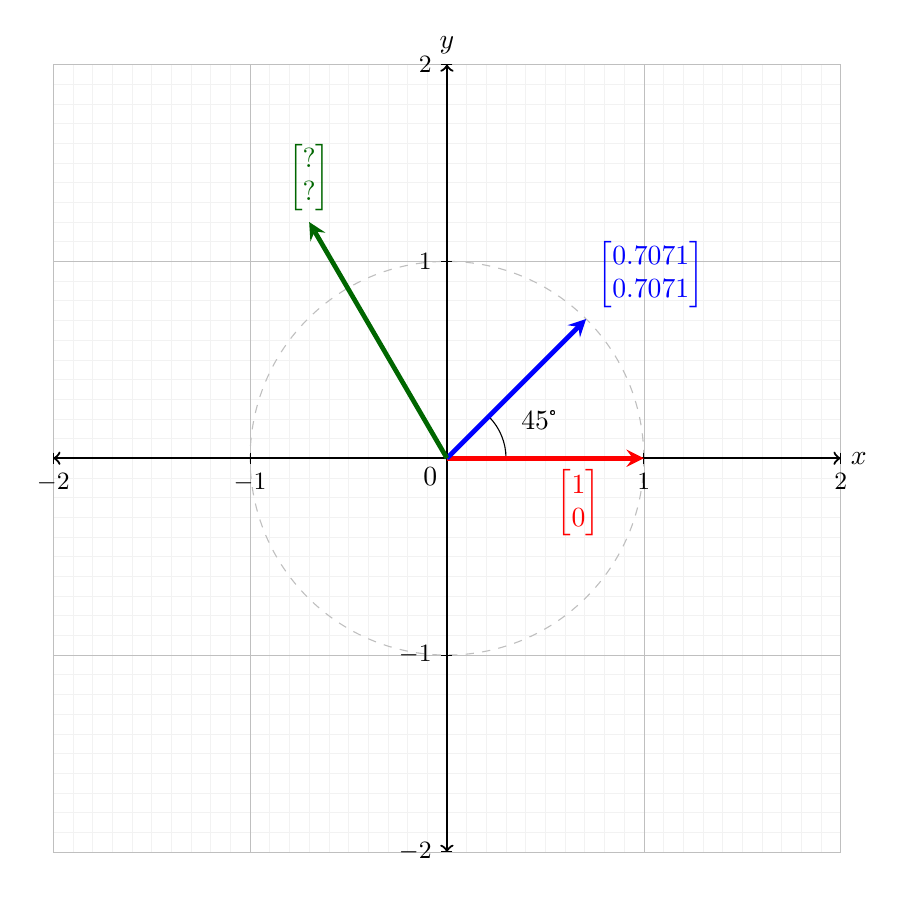
\begin{tikzpicture}[x=2.5cm,y=2.5cm]
        \coordinate (Origin) at (0, 0);
        \coordinate (R) at (0.7071, 0.7071);
        \coordinate (P) at (1, 0);

        % Draw grid
        \draw[gray!10, very thin, step=0.1] (-2, -2) grid (2, 2);
        \draw[gray!50, very thin, step=1] (-2, -2) grid (2, 2);

        \draw[gray!50, dashed] (0, 0) circle (1);

        % Draw tick marks on the axes
        \foreach \x in {-2, -1, 1, 2}
        \draw (\x, 2pt) -- (\x, -2pt) node[below] {\small $\x$};
        \foreach \y in {-2, -1, 1, 2}
        \draw (2pt, \y) -- (-2pt, \y) node[left] {\small $\y$};

        \node[below left] at (0, 0) {$0$};

        % Draw Cartesian axes
        \draw[<->, thick] (-2, 0) -- (2, 0) node[right] {$x$};
        \draw[<->, thick] (0, -2) -- (0, 2) node[above] {$y$};

        \pic[draw, angle radius=0.75cm, angle eccentricity=1.7, "$45$\textdegree"] {angle=P--Origin--R};

        % Draw red vector arrow [1, 0]
        \draw[->, red, line width=0.6mm, >={stealth}] (0, 0) -- (P) node[midway, below right] {$\begin{bmatrix}1 \\ 0\end{bmatrix}$};

        % Draw blue vector arrow [0.7071, 0.7071]
        \draw[->, blue, line width=0.6mm, >={stealth}] (0, 0) -- (R) node[above right]
            {$\begin{bmatrix}0.7071 \\ 0.7071\end{bmatrix}$};

        \draw[->, black!60!green, line width=0.6mm, >={stealth}] (0, 0) -- (-0.7, 1.2) node[above]
            {$\begin{bmatrix}? \\ ?\end{bmatrix}$};

    \end{tikzpicture}
    \caption{ Apparent rotation of red vector $\begin{bmatrix}1 \\ 0\end{bmatrix}$ by
        45\textdegree \space anti-clockwise to blue vector }
    \label{2d_rot}
\end{figure}

From Figure \ref{2d_rot}, it may seem like calculating this rotation is trivial
by using the trigonometric functions: for any angle $\theta$, the rotation of
$\begin{bmatrix}1 \\ 0\end{bmatrix}$ is equal to $\begin{bmatrix}\cos\theta \\
        \sin\theta\end{bmatrix}$. \vspace{0.2cm}

Indeed, this is the case for the simple example above, but the applicability of
this model quickly breaks down once the complexity is increased. For example,
rotating the green vector about a point different to the origin by using this
model is difficult to imagine. Furthermore, if one was to go beyond rotation,
how could the red vector be transformed into the green vector? \\

Linear transformation using matrices elegantly deals with these problems by
introducing one concept - instead of transforming each individual vector,
transform the axes themselves. \\

\begin{figure}[H]
    \centering
    \vspace{0.5cm}
    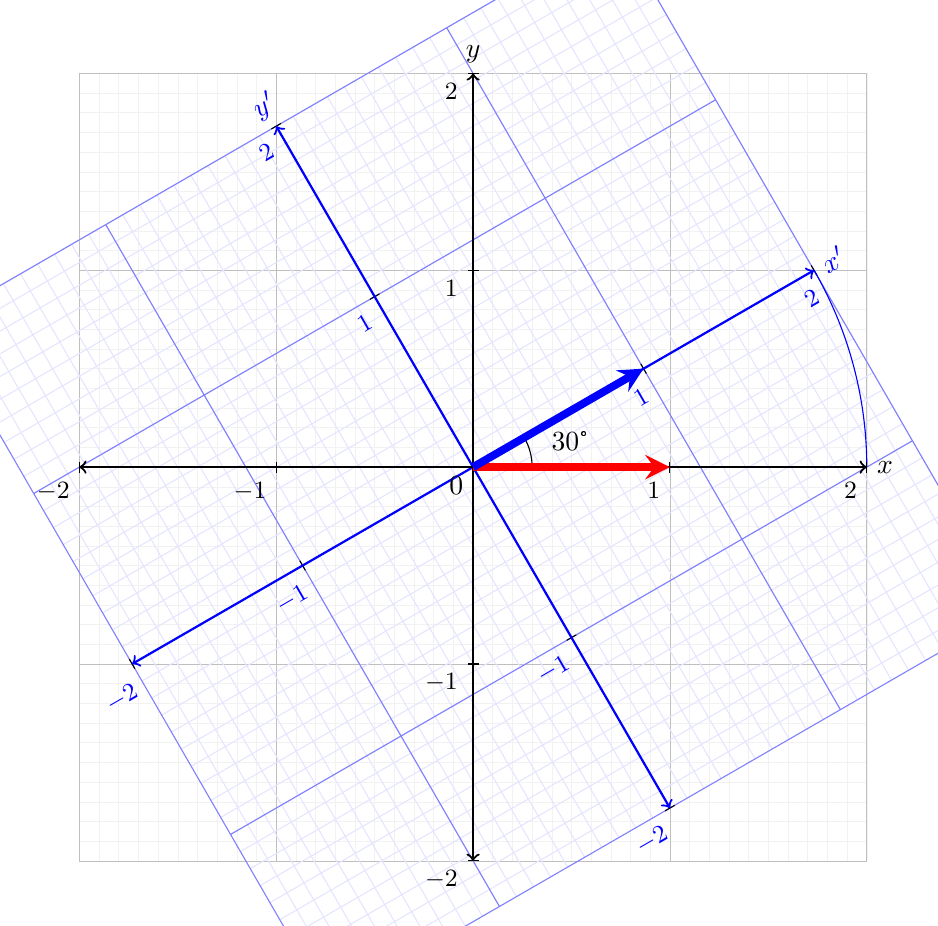
\begin{tikzpicture}[x=2.5cm,y=2.5cm]
        \coordinate (Origin) at (0, 0);
        \coordinate (R) at (0.8660, 0.5);
        \coordinate (P) at (1, 0);

        % Draw grid
        \draw[gray!10, very thin, step=0.1] (-2, -2) grid (2, 2);
        \draw[gray!50, very thin, step=1] (-2, -2) grid (2, 2);

        % 45deg
        \rotatebox{30}{
            \draw[step=0.1, blue!10, very thin, thin] (-2,-2) grid (2,2);
            \draw[step=1, blue!50, very thin, thin] (-2,-2) grid (2,2);

            \foreach \x in {-2, -1, 1, 2}
            \draw (\x, 2pt) -- (\x, -2pt) node[blue, below left] {\small $\x$};
            \foreach \y in {-2, -1, 1, 2}
            \draw (2pt, \y) -- (-2pt, \y) node[blue, below left] {\small $\y$};

            \draw[<->, blue, thick] (-2, 0) -- (2, 0) node[right] {$x'$};
            \draw[<->, blue, thick] (0, -2) -- (0, 2) node[above] {$y'$};
        }

        \pic[draw, blue, angle radius=5cm] {angle=P--Origin--R};

        % Draw tick marks on the axes
        \foreach \x in {-2, -1, 1, 2}
        \draw (\x, 2pt) -- (\x, -2pt) node[below left] {\small $\x$};
        \foreach \y in {-2, -1, 1, 2}
        \draw (2pt, \y) -- (-2pt, \y) node[below left] {\small $\y$};

        \node[below left] at (0, 0) {$0$};

        % Draw Cartesian axes
        \draw[<->, thick] (-2, 0) -- (2, 0) node[right] {$x$};
        \draw[<->, thick] (0, -2) -- (0, 2) node[above] {$y$};

        \pic[draw, angle radius=0.75cm, angle eccentricity=1.7, "$30$\textdegree"] {angle=P--Origin--R};

        % Draw red vector arrow [1, 0]
        \draw[->, red, line width=1mm, >={stealth}] (0, 0) -- (P);

        % Draw blue vector arrow [0.7071, 0.7071]
        \draw[->, blue, line width=1mm, >={stealth}] (0, 0) -- (R);
    \end{tikzpicture}

    \vspace{1.5cm}
    \caption{ Overlay of new cartesian plane (blue) with axes $x'$ and $y'$
        rotated 30\textdegree \space anti-clockwise relative to the original. }
    \label{2d_axis_rot}
\end{figure}

In Figure \ref{2d_axis_rot}, the blue vector's coordinates on the rotated axes
are identical to the red vector's coordinates on the original - both are
$\begin{bmatrix}1 \\ 0\end{bmatrix}$. In fact, any one point on the original
axis has a counterpart on the rotated axis which corresponds to the rotation of
that point about the origin by $30$\textdegree. If one examines the coordinates
of the blue vector $b$ on the original axes, it becomes evident that
$
    \vec{b}
    =
    \begin{bmatrix}
        0.8660 \hdots \\ 0.5
    \end{bmatrix}
    =
    \begin{bmatrix}
        \cos 30^\circ \\
        \sin 30^\circ
    \end{bmatrix}
$, which aligns with findings from the trigonometric model. \\

Another invaluable benefit of this method is that one may also choose to rotate
the axes about a different point to the origin, and observe the correct
off-centric rotations for vectors without any changes to how the model is
evaluated. Extrapolating this to three dimensions yields immeasurable savings in
complexity and extra calculations which are expensive for computers to do. \\

\begin{figure}[H]
    \centering
    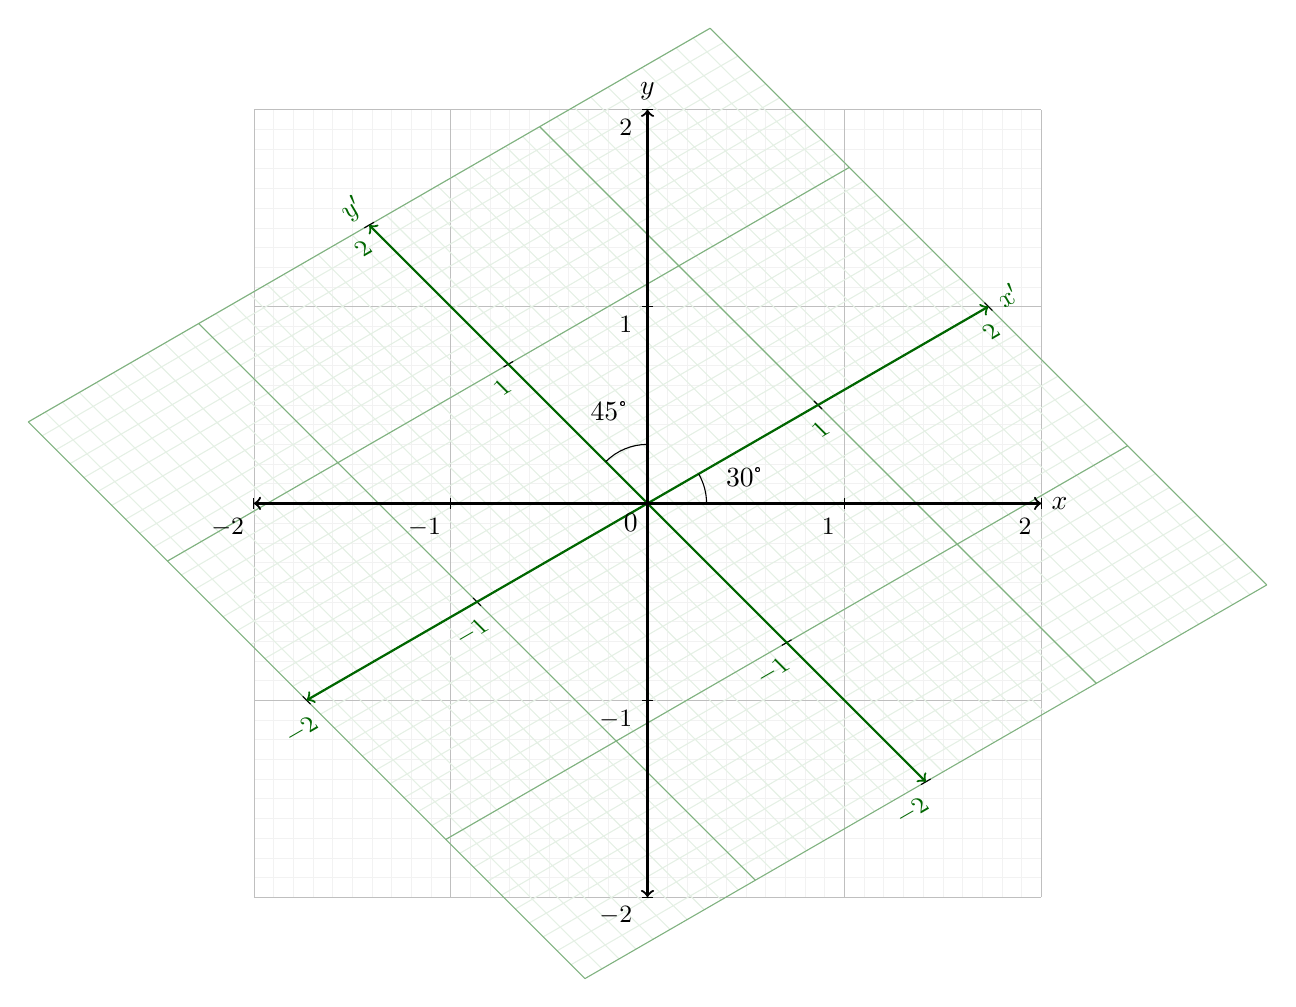
\begin{tikzpicture}[x=2.5cm,y=2.5cm]
        \coordinate (Origin) at (0, 0);
        \coordinate (R) at (0.8660, 0.5);
        \coordinate (P) at (1, 0);
        \coordinate (R2) at (-0.707, 0.707);
        \coordinate (P2) at (0, 1);

        % Draw grid
        \draw[gray!10, very thin, step=0.1] (-2, -2) grid (2, 2);
        \draw[gray!50, very thin, step=1] (-2, -2) grid (2, 2);

        \begin{scope}[cm={0.8660, 0.5, -0.707, 0.707,(0,0)}]
            \draw[step=0.1, black!60!green!10, very thin, thin] (-2,-2) grid (2,2);
            \draw[step=1, black!60!green!50, very thin, thin] (-2,-2) grid (2,2);

            \foreach \x in {-2, -1, 1, 2}
            \draw (\x, 2pt) -- (\x, -2pt) node[black!60!green, below left, transform shape] {\small $\x$};
            \foreach \y in {-2, -1, 1, 2}
            \draw (2pt, \y) -- (-2pt, \y) node[black!60!green, below left, transform shape] {\small $\y$};

            \draw[<->, black!60!green, thick] (-2, 0) -- (2, 0) node[right, transform shape] {$x'$};
            \draw[<->, black!60!green, thick] (0, -2) -- (0, 2) node[above, transform shape] {$y'$};

            % \node[circle, fill=black!60!green, inner sep=0pt, minimum size=5pt, transform shape] 
            %     at (1, 0) {};
            % \node[black!60!green, transform shape, above right] at (1, 0) {A'$(1, 0)$};

            % \node[circle, fill=black!60!green, inner sep=0pt, minimum size=5pt, transform shape] 
            %     at (0, 1) {};
            % \node[black!60!green, transform shape, above right] at (0, 1) {B'$(0, 1)$};
        \end{scope}

        % Draw tick marks on the axes
        \foreach \x in {-2, -1, 1, 2}
        \draw (\x, 2pt) -- (\x, -2pt) node[below left] {\small $\x$};
        \foreach \y in {-2, -1, 1, 2}
        \draw (2pt, \y) -- (-2pt, \y) node[below left] {\small $\y$};

        \node[below left] at (0, 0) {$0$};

        % Draw Cartesian axes
        \draw[<->, thick] (-2, 0) -- (2, 0) node[right] {$x$};
        \draw[<->, thick] (0, -2) -- (0, 2) node[above] {$y$};

        \pic[draw, angle radius=0.75cm, angle eccentricity=1.7, "$30$\textdegree"] {angle=P--Origin--R};
        \pic[draw, angle radius=0.75cm, angle eccentricity=1.7, "$45$\textdegree"] {angle=P2--Origin--R2};

        % \node[circle, fill, inner sep=0pt, minimum size=5pt] 
        %     at (1, 0) {};
        % \node[above right] at (1, 0) {A$(1, 0)$};

        % \node[circle, fill, inner sep=0pt, minimum size=5pt] 
        %     at (0, 1) {};
        % \node[above right] at (0, 1) {B$(0, 1)$};

        % \draw[->, red, line width=0.6mm, >={stealth}] (0, 0) -- (P);
        % \draw[->, black!60!green, line width=0.6mm, >={stealth}] (0, 0) -- (R);

        % \draw[->, red, line width=0.6mm, >={stealth}] (0, 0) -- (P2);
        % \draw[->, black!60!green, line width=0.6mm, >={stealth}] (0, 0) -- (R2);
    \end{tikzpicture}
    \caption{ Overlay of new cartesian plane (green) with axes $x'$ and $y'$
        rotated 30\textdegree\space anti-clockwise and 45\textdegree\space anti-clockwise respectively. }
    \label{2d_axis_shear}
\end{figure}

Figure \ref{2d_axis_shear} depicts what is known as a "shear". It occurs when
each axis is rotated by a different angle, and results in warping of the
transformed vectors, evident by the asymmetric appearance of the graph. If you
were interested in going beyond rotation, there is an opportunity to translate,
dilate and shear the axes to achieve various effects like the one depicted.\\

The elegance in this model comes from how one such transformation is actually
computed. The first step to this is determining the direction and dilation of the
transformed axes by examining what happens to the vectors $\begin{bmatrix} 1 \\
        0\end{bmatrix}$ and $\begin{bmatrix} 0 \\
        1\end{bmatrix}$ after the transformation. If the magnitude of any one of these
vectors changes, that means that the respective axis has been dilated by a
factor of the magnitude. If the direction changes, that means that that axis has
been rotated. By knowing the final position of these two vectors after a
transformation, the transformation that took place can be reconstructed and
applied to more points. \\

\pagebreak

The extremely useful tool that bridges the gap between this theory of axis
shifting and mathematics is called a transformation matrix. 2D Transformation
matrices are constructed by taking the vectors found above and storing them in a
single 2$\times$2 matrix:

Let $x$ be the post-transform position of $\begin{bmatrix} 1 \\ 0
    \end{bmatrix}$, where $\vec{x} = \begin{bmatrix} x_x \\ x_y
    \end{bmatrix}$, and let $y$ be the post-transform position of
$\begin{bmatrix} 0 \\ 1 \end{bmatrix}$, where $\vec{y} =
    \begin{bmatrix}y_x \\ y_y \end{bmatrix}$. The transformation matrix
$M$ is described by $ M = \begin{bmatrix} x_x & y_x \\
                x_y & y_y
    \end{bmatrix}$.\\

The transformation $T_M(\vec{v})$ of $\vec{v}$ by matrix $M$ can then be
described as

\begin{align*}
    T_M(\vec{v}) = M\vec{v} = 
    \begin{bmatrix}
        x_x & y_x \\
        x_y & y_y
    \end{bmatrix}
    \begin{bmatrix}
        v_x \\
        v_y
    \end{bmatrix}
    =
    \begin{bmatrix}
        x_xv_x + y_xv_y \\
        x_yv_x + y_yv_y
    \end{bmatrix}
\end{align*}

If $\vec{x}$ and $\vec{y}$ do not change after a transformation, they would be
equal to $\begin{bmatrix} 1 \\ 0 \end{bmatrix}$ and $\begin{bmatrix} 0 \\ 1
    \end{bmatrix}$ respectively. From this, a transformation matrix which does nothing
(called the "identity") $M_0$ can be constructed in the form of
$
    M_0 = \begin{bmatrix}
        1 & 0 \\
        0 & 1
    \end{bmatrix}
$. In this case, $T_{M_0}(\vec{v}) = \begin{bmatrix}
        (1)v_x + (0)v_y \\
        (0)v_x + (1)v_y \end{bmatrix} = \begin{bmatrix} v_x \\
        v_y
    \end{bmatrix} = \vec{v}$ \\\\

Considering the point $\begin{bmatrix} 1 \\ 0 \end{bmatrix}$ on a unit circle,
a rotation by $\theta$ would be represented as $\begin{bmatrix} \cos\theta \\
\sin\theta \end{bmatrix}$. Likewise, the rotation of the point $\begin{bmatrix}
0 \\ 1 \end{bmatrix}$ is equrivalent to $\begin{bmatrix} -\sin\theta \\
\cos\theta \end{bmatrix}$. Hence, a 2D transformation matrix $R(\theta)$ can be
constructed so that it rotates the 2D axes by any angle $\theta$. This is what is
known as a rotation matrix.

\begin{align*}
    R(\theta) & = \begin{bmatrix}
                      \cos\theta & -\sin\theta \\
                      \sin\theta & \cos\theta
                  \end{bmatrix}
\end{align*}

% TODO: needs clarity
You can combine different linear transformations by multiplying a vector by
multiple transformation matrices sequentially. For example, you might choose to
apply a shear or a scale to your points before rotating them. This property
applies to both two and three dimensional transformation matrices. Because of
this versatility, transformation matrices are very easy to work with and
integrate into more complex operations. \\

It is important to note that matrix multiplication is not commutative, and hence
it is important to always multiply matrices in a right-to-left order: if one
wanted to apply the linear transformations $T_1 \to T_2 \to T_3$ on vector
$\vec{v}$, the correct multiplication would be $T_3T_2T_1\vec{v}$.

\pagebreak
\subsection{In three dimensions}
Now that we have established basic intuition on what 2D matrices actually do, we
can extend the established observations to three dimensions. \\

In 3D, there are now three axes which must be kept track of:
\begin{itemize}[leftmargin=2cm]
    \item X (left $\leftrightarrow$ right)
    \item Y (up $\updownarrow$ down)
    \item Z (forward $\neswarrow$ back)
\end{itemize}

The identity vectors $\vec{x}_0$, $\vec{y}_0$ and $\vec{z}_0$ in three
dimensions, like we saw with 2D, have a magnitude of $1$ and lie on the axis
they represent.

\begin{align*}
    \vec{x}_0 = \begin{bmatrix} 1 \\ 0 \\ 0 \end{bmatrix}
    \quad
    \vec{y}_0 = \begin{bmatrix} 0 \\ 1 \\ 0 \end{bmatrix}
    \quad
    \vec{z}_0 = \begin{bmatrix} 0 \\ 0 \\ 1 \end{bmatrix}
\end{align*} \\

The 3D transformation defines the transition from the identity vectors into ones
($\vec{x}$, $\vec{y}$ and $\vec{z}$) with potentially different magnitude and
direction, signifying reoriented axes.

\begin{align*}
    \vec{x} = \begin{bmatrix}
                  {x}_x \\ {y}_x \\ {z}_x
              \end{bmatrix}
    \quad
    \vec{y} = \begin{bmatrix}
                  {x}_y \\ {y}_y \\ {z}_y
              \end{bmatrix}
    \quad
    \vec{z} = \begin{bmatrix}
                  {x}_z \\ {y}_z \\ {z}_z
              \end{bmatrix}
\end{align*}

Changing the magnitude and/or direction of these vectors results in various effects
on the 3D space, similar to how this works in two dimensions. Individually
changing any one or two of these vectors results in the three dimensional
equrivalent of shear called "deformation". This property is often used in 3D
animation to compress or stretch objects -- a bouncing ball, for example. \\

As before, constructing a matrix out of these vectors allows us to leverage
matrix multiplication to transform points. A 3$\times$3 matrix $M$ can now be
constructed to represent a 3D transformation using the above axes. Let the
identity of $M$ be $M_0$.

\begin{align*}
    M = \begin{bmatrix}
            {x}_x & {y}_x & {z}_x \\
            {x}_y & {y}_y & {z}_y \\
            {x}_z & {y}_z & {z}_z
        \end{bmatrix} \quad\therefore\quad M_0 = \begin{bmatrix}
                                                     1 & 0 & 0 \\
                                                     0 & 1 & 0 \\
                                                     0 & 0 & 1
                                                 \end{bmatrix}
\end{align*}

For a transformation $T_M(\vec{v})$ on $\vec{v} = \begin{bmatrix}
        v_x \\
        v_y \\
        v_z \end{bmatrix}$ by matrix $M$,

\begin{align*}
    T_M(\vec{v}) = M\vec{v} = \begin{bmatrix}
                                  {x}_x & {y}_x & {z}_x \\
                                  {x}_y & {y}_y & {z}_y \\
                                  {x}_z & {y}_z & {z}_z
                              \end{bmatrix}
    \begin{bmatrix}
        v_x \\
        v_y \\
        v_z
    \end{bmatrix}
    =
    \begin{bmatrix}
        x_x v_x + y_x v_y + z_x v_y \\
        x_y v_x + y_y v_y + z_y v_y \\
        x_z v_x + y_z v_y + z_z v_y \\
    \end{bmatrix}
\end{align*}

In our case, we seek to perform a rotation on a set of 3D points, meaning that
we would need a form for a 3D rotation matrix. Like observed in the 2D case, a
rotation could affect more than one axis, and so it is important to consider the
matrix as a whole. Historically, many different ways of constructing rotation
matrices have been shown, each with their benefits and downsides. In a sense,
rotation matrices are not an entirely independent method of performing rotation,
but are rather an underlying infrastructure for other methods to use.

\subsection{Construction from Euler angles}

\subsubsection{Concept}
In real life, it is practical to represent rotations with easily measurable
metrics, like angles. Aircraft and watercraft make extensive use of yaw, pitch
and roll angles in instrumentation to aid their pilots in judging the
orientation of the craft. Yaw indicates a horizontal swivel, or a "heading",
pitch indicates the angle of the nose relative to the horizon, and roll
indicates how much the plane is turned about the forward axis. Figure
\ref{yawpitchroll} demonstrates this in terms of an $x$, $y$ and $z$ axis. In
aircraft, $y$ axis here can be considered as the "front" of the craft. \\

\begin{figure}[H]
    \centering
    \tdplotsetmaincoords{70}{-45}
    \begin{tikzpicture}[x=0.5cm,y=0.5cm,z=0.3cm,>=stealth,tdplot_main_coords]
        \coordinate (X) at (3,0,0);
        \coordinate (Y) at (0,3,0);
        \coordinate (Z) at (0,0,3);

        \draw[->, black!30!red] (0,0,0) -- (X) node[right] {$x$};
        \draw[->, black!30!blue] (0,0,0) -- (Y) node[left] {$y$};
        \draw[->, black!30!green] (0,0,0) -- (Z) node[above] {$z$};

        \node[red] at (2.25,0,0.8) {$pitch$};
        \begin{scope}[canvas is zy plane at x=2.5]
            \draw[red, dashed] (0,0) circle (0.3);
        \end{scope}

        \node[black!30!green] at (1,0,2.25) {$yaw$};
        \begin{scope}[canvas is xy plane at z=2.5]
            \draw[black!30!green, dashed] (0,0) circle (0.3);
        \end{scope}

        \node[blue] at (0.1,2.25,0.6) {$roll$};
        \begin{scope}[canvas is xz plane at y=2]
            \draw[blue, dashed] (0,0) circle (0.3);
        \end{scope}


    \end{tikzpicture}
    \caption{Yaw pitch and roll}
    \label{yawpitchroll}
\end{figure}

Euler angles are based around this concept. A set of Euler angles is a 3D vector
containing the yaw, pitch and roll of an object around a reference frame. In the
example of aircraft, the reference frame is usually the surface of the Earth. In
space, it is usually a prominent constellation or celestial object. \\

As this system of representing rotation is simple, measurable and intuitive for
humans to use, one of the main ways of constructing a rotation matrix is through
Euler angles.

\pagebreak
\subsubsection{Deriving rotation matrices for each angle}
\label{section_deriving_rot_for_each_angle}
Consider rotating the 3D identity axes $\vec{x}_0$, $\vec{y}_0$ and $\vec{z}_0$
by $\theta$ around the X axis. Let the matrix that describes this rotation in
terms of $\theta$ be $R_x(\theta)$. After the transformation, let the identity
vectors' new positions be $\vec{x}_r$, $\vec{y}_r$ and $\vec{z}_r$. \\

% TODO: insert figure

\begin{figure}[H]
    \centering
    \tdplotsetmaincoords{70}{50}
    \begin{tikzpicture}[x=0.5cm,y=0.5cm,z=0.3cm,>=stealth,tdplot_main_coords]
        \coordinate (X) at (5,0,0);
        \coordinate (Y) at (0,3,0);
        \coordinate (Z) at (0,0,3);

        \draw[->, red] (0,0,0) -- (X) node[right] {$\vec{x}_r = R_{x}(\theta)\cdot \vec{x}_0 = x_0$};
        \draw[->, blue] (0,0,0) -- (Y) node[right] {$y_0$};
        \draw[->, black!60!green] (0,0,0) -- (Z) node[above] {$z_0$};

        \begin{scope}[canvas is zy plane at x=0]
            \draw[dashed, darkgray] (0,0) circle (3);
            \draw[->, blue, dashed] (0,0) -- ({sin(20)*3}, {cos(20)*3}) node[right] {$\vec{y}_r = R_{x}(\theta)\cdot \vec{y}_0$};
            \draw[->, black!60!green, dashed] (0,0) -- ({sin(110)*3}, {cos(110)*3}) node[above left] {$\vec{z}_r = R_{x}(\theta)\cdot \vec{z}_0$};

            \draw[black!30!blue] (0.26,1.5) node {$\theta$};
            \draw[black!80!green] (1.5,-0.26) node {$\theta$};
        \end{scope}

    \end{tikzpicture}
    \caption{Rotation around the X-axis by angle $\theta$. $\vec{x}_r$,
        $\vec{y}_r$ and $\vec{z}_r$ represent the identity vectors after the
        transformation by $R_x(\theta)$ where $\vec{x}_0 \to \vec{x}_r$,
        $\vec{y}_0 \to \vec{y}_r$ and $\vec{z}_0 \to \vec{z}_r$.}
    \label{3d_euler_rot_x}
\end{figure}

In Figure \ref{3d_euler_rot_x}, the rotation $R_x(\theta)$ could be represented
as

\begin{align*}
    R_x(\theta) = \begin{bmatrix}
        {x}_{rx} & {y}_{rx} & {z}_{rx} \\
        {x}_{ry} & {y}_{ry} & {z}_{ry} \\
        {x}_{rz} & {y}_{rz} & {z}_{rz}
    \end{bmatrix}
\end{align*}\\

From Figure \ref{3d_euler_rot_x} it becomes apparent that points colinear with
$\vec{x}_0$ do not move at all, because in this case the rotation is happening
along the X-axis. Hence,

\begin{align*}
    \vec{x}_r = \vec{x}_0 = \begin{bmatrix} 1 \\
                              0 \\ 0\end{bmatrix}
\end{align*}

Points colinear with the Y axis get rotated around a unit circle in the YZ plane
(pictured in Figure \ref{3d_euler_rot_x}). Hence, $\vec{y}_r$ is described with
the trigonometric functions $\cos \theta$ and $\sin \theta$ as its Y and Z
components. The rotation of $\vec{z}_r$ can be derived similarly.

\begin{align*}
    \vec{y}_r = \begin{bmatrix} 0 \\ \cos\theta \\ \sin\theta
                      \end{bmatrix}
    \quad
    \vec{x}_r
    = \begin{bmatrix}
          0           \\
          -\sin\theta \\
          \cos\theta
      \end{bmatrix}
\end{align*}

Combining $\vec{x}_r, \vec{y}_r$ and $\vec{z}_r$ yields the rotation matrix
$R_x(\theta)$ for rotations around the X-axis.

\begin{align*}
    R_x(\theta)
    = \begin{bmatrix}
          1 & 0          & 0           \\
          0 & \cos\theta & -\sin\theta \\
          0 & \sin\theta & \cos\theta
      \end{bmatrix}
\end{align*}

A  similar process can be followed to derive the rotation matrices by the Y and
Z axes, so it has been omitted for brevity. The only thing that changes in the
derivation process is that the plane of the circle follows the two axes perpendicular to
the rotation axis.

\begin{align*}
    R_y(\theta) = \begin{bmatrix}
                      \cos \theta  & 0 & \sin \theta \\
                      0            & 1 & 0           \\
                      -\sin \theta & 0 & \cos \theta
                  \end{bmatrix}
    \quad
    R_z(\theta) = \begin{bmatrix}
                      \cos \theta & -\sin \theta & 0 \\
                      \sin \theta & \cos \theta  & 0 \\
                      0           & 0            & 1
                  \end{bmatrix}
\end{align*}

\subsubsection{Multiplication}

For the Euler angles $\alpha$, $\beta$ and $\gamma$ representing yaw, pitch and
roll respectively, it is now possible to compute a general rotation matrix by
first constructing each individual matrix, then multiplying them. Effectively,
this applies the rotation $R_x(\alpha)$ followed by $R_y(\beta)$ and finally
$R_z(\gamma)$.

\begin{align*} \\
    R(\alpha, \beta, \gamma) & = R_z(\gamma) R_y(\beta) R_x(\alpha)                                                                                                \\
                             & = \begin{bmatrix}
                                     \cos \gamma & -\sin \gamma & 0 \\
                                     \sin \gamma & \cos \gamma  & 0 \\
                                     0           & 0            & 1 \\
                                 \end{bmatrix}
    \begin{bmatrix}
        \cos \beta  & 0 & \sin \beta \\
        0           & 1 & 0          \\
        -\sin \beta & 0 & \cos \beta \\
    \end{bmatrix}
    \begin{bmatrix}
        1 & 0           & 0            \\
        0 & \cos \alpha & -\sin \alpha \\
        0 & \sin \alpha & \cos \alpha  \\
    \end{bmatrix}                                                                                                                                 \\
                             & = \begin{bmatrix}
                                     \cos\beta\cos\gamma & \sin\alpha\sin\beta\cos\gamma - \cos\alpha\sin\gamma & \cos\alpha\sin\beta\cos\gamma + \sin\alpha\sin\gamma \\
                                     \cos\beta\sin\gamma & \sin\alpha\sin\beta\sin\gamma + \cos\alpha\cos\gamma & \cos\alpha\sin\beta\sin\gamma - \sin\alpha\cos\gamma \\
                                     -\sin\beta          & \sin\alpha\cos\beta                                  & \cos\alpha\cos\beta                                  \\
                                 \end{bmatrix}
\end{align*} \\

As matrix multiplication does not commute, it is not always the case that
rotating by an axis A, then rotating by B would be the same as rotating first by
axis B, then by A. Hence, it is important to note that the order of
multiplication of $R_z$, $R_y$ and $R_x$ produces a unique final rotation. For
the rest of the investigation, the $x \to y \to z$ rotation order seen above
will be used. This is alternatively called the ZYX Tait-Bryan order.

\pagebreak
\subsection{The gimball lock problem}
There is one large problem with constructing rotation matrices from Euler
angles. Suppose you rotated an object with the Euler angles
$\alpha$, $\beta$ and $\gamma$, where $\beta=\frac{\pi}{2}$

\begin{align*} \\
    R(\alpha, \frac{\pi}{2}, \gamma)
     & = \begin{bmatrix}
             \cos\frac{\pi}{2}\cos\gamma & \sin\alpha\sin\frac{\pi}{2}\cos\gamma - \cos\alpha\sin\gamma & \cos\alpha\sin\frac{\pi}{2}\cos\gamma + \sin\alpha\sin\gamma \\
             \cos\frac{\pi}{2}\sin\gamma & \sin\alpha\sin\frac{\pi}{2}\sin\gamma + \cos\alpha\cos\gamma & \cos\alpha\sin\frac{\pi}{2}\sin\gamma - \sin\alpha\cos\gamma \\
             -\sin\frac{\pi}{2}          & \sin\alpha\cos\frac{\pi}{2}                                  & \cos\alpha\cos\frac{\pi}{2}                                  \\
         \end{bmatrix}
    \\
     & = \begin{bmatrix}
             0  & \sin\alpha\cos\gamma - \cos\alpha\sin\gamma & \cos\alpha\cos\gamma + \sin\alpha\sin\gamma \\
             0  & \sin\alpha\sin\gamma + \cos\alpha\cos\gamma & \cos\alpha\sin\gamma - \sin\alpha\cos\gamma \\
             -1 & 0                                           & 0                                           \\
         \end{bmatrix}
    \\
     & = \begin{bmatrix}
             0  & \sin(\alpha - \gamma) & \cos(\alpha - \gamma)  \\
             0  & \cos(\alpha - \gamma) & -\sin(\alpha - \gamma) \\
             -1 & 0                     & 0                      \\
         \end{bmatrix}
\end{align*} \\

Let $\alpha - \gamma = \theta$. The rotation matrix $R$ now becomes $R(\theta) =
    \begin{bmatrix} 0  & \sin\theta & \cos\theta  \\
    0  & \cos\theta & -\sin\theta \\
    -1 & 0          & 0           \\
\end{bmatrix}$.\\
By inspecting this matrix, we find that:

\begin{itemize}[leftmargin=2cm]
    \item $\vec{x_0}$ will always transform to $-\vec{z_0}$. This means that
    this is the axis around which rotation occurs by angle $\theta$.
    \item $\vec{y}$ and $\vec{z}$ revolve around a unit circle in the YX plane
    by angle $\theta$.
    \item This matrix is entirely in terms of $\theta$. It does not matter
    whether the $\alpha$ or $\gamma$ is changed, the resulting rotation will always
    be around the $-\vec{z_0}$ axis.
\end{itemize}

Hence, this shows that when $\beta = \frac{\pi}{2}$, the rotation matrix
actually loses one degree of rotational freedom entirely as $\alpha$ and
$\gamma$ describe rotation about the same axis. In fact, the same can be shown
for the case where one of $\alpha$, $\beta$ or $\gamma$ is equal to
$\frac{a\pi}{2}$ where $a = (2b+1)$, $b \in \mathbb{Z}$. \\

This phenomenon is known as "gimball lock". It is widely considered to be one of
the largest issues with using Euler angles for rotation. It is significant
because it means that for specific angles of rotation, the system can actually
lose the ability to freely rotate, and may even be unable to escape the gimball
lock. \\

\pagebreak

\begin{figure}[H]
    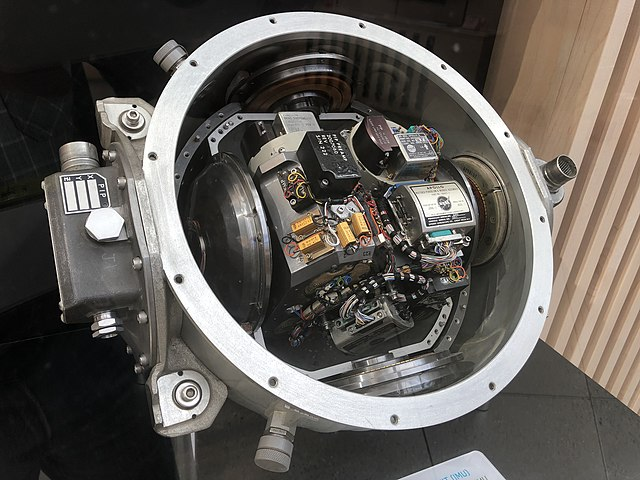
\includegraphics[width=8cm]{res/apollo_imu.jpg}
    \centering
    \caption{The Apollo 11 "Inertial Measurement Unit" responsible for guidance \& orientation of the spacecraft in space.}
\end{figure}

One of the most famous examples of gimball lock in action was during the 1969
Apollo 11 manned mission to the moon. The Apollo 11 spacecraft was equipped with
an "Inertial Measurement Unit" which was responsible for measuring the
orientation of the spacecraft in space. This was done using three gyroscopes,
each of which measured the rotation of the spacecraft in terms of yaw, pitch and
roll relative to the craft's starting position. Mechanically, these gyroscopes,
too undergo gimball lock when the spacecraft is oriented at specific angles
resulting in complete disorientation of the guidance unit. This happened
in-flight during the actual mission, meaning that the unit had to be manually
moved out of the gimbal lock position using the stars as a reference, in order
to regain the lost degree of freedom. \\

This fundamental flaw with Euler angles demonstrates how despite their
simplicity and intuitiveness, they clearly leave a lot to be desired for
rigorously representing 3D rotations. \\

% \subsection{The spherical linear interpolation problem}

\section{Improving on Euler angles with Quaternions}
In 1843, Irish mathematician Sir William Rowan Hamilton proposed an alternative
way to represent 3D rotation by using four dimensional imaginary numbers called
"quaternions". Quaternions allow us to rotate any point vector around any axis
by a certain angle. This method of rotation is not anything special in
particular - in fact, rotating around the X, Y and Z axes individually has
already been explored in section \ref{section_deriving_rot_for_each_angle}.

\subsection{Standard Form}
Quaternions, like complex numbers, are defined with "real" and "imaginary"
parts, and are essentially an extension of the complex numbers to four
dimensions. The set of all quaternions is known as $\mathbb{H}$, named after the
last initial of the Irish mathematician William Rowan Hamilton. Algebraically, a
quaternion $q$ can be defined in terms of the coefficients of its terms:

\begin{align*}
    q = a + bi + cj + dk \quad a, b, c, d \in \mathbb{R}
\end{align*}

$i$, $j$ and $k$, called "basic quaternions", do not have an explicit definition
of their value but are rather defined expressly in terms of the way they
interact with each other in that they must satisfy the equality

\begin{align*}
    i^2 = j^2 = k^2 = ijk = -1
\end{align*}

\subsection{Basic Quaternions}

\subsubsection{Multiplying by Real Numbers}
For any $n \in \mathbb{R}$, it is defined that $in = ni$, $jn = nj$ and $kn =
    nk$. Hence, for any $q \in \mathbb{H}$, $qn = nq$. Quaternion multiplication by
real numbers does, in fact, commute.

\subsubsection{Multiplication by other basic quaternions}
Hamilton's quaternion definition can then be used to derive the multiplicative
interactions between $i$, $j$ and $k$:

% ij & jk
\begin{align*}
     &
    \begin{aligned}
        ijk    & = k^2   \\
        ijk^2  & = k^2k  \\
        ij(-1) & = (-1)k \\
        ij     & = k
    \end{aligned}
     &
    \begin{aligned}
        ijk    & = i^2         \\
        i^2 jk & = i \cdot i^2 \\
        (-1)jk & = i(-1)       \\
        jk     & = i
    \end{aligned}
\end{align*}

% kj and ji
\begin{align*}
     &
    \begin{aligned}
        i  & = jk   \\
        ji & = j^2k \\
        ji & = -k
    \end{aligned}
     &
    \begin{aligned}
        k  & = ij   \\
        kj & = ij^2 \\
        kj & = -i
    \end{aligned}
\end{align*}

% ki & ik
\begin{align*}
     &
    \begin{aligned}
        ij     & = k     \\
        kij    & = k^2   \\
        kij^2  & = k^2j  \\
        ki(-1) & = (-1)j \\
        ki     & = j
    \end{aligned}
     &
    \begin{aligned}
        k  & = ij   \\
        ik & = i^2j \\
        ik & = -j
    \end{aligned}
\end{align*}

An important concept becomes apparent from the above calculations - quaternion
multiplication by other quaternions is not commutative, that is, it can be the
case that $q_1q_2 \neq q_2q_1$ where $ q_1,q_2 \in \mathbb{H}$. For example, it
is seen above that while $ij = k$, $ji = -k$. \\

The multiplication table of basic quaternions is hence formed:

\begin{center}
    \doublespacing
    \begin{tabular}{ | c | c | c | c | }
        \hline
        $\times$ & $i$  & $j$  & $k$  \\
        \hline
        $i$      & $-1$ & $-k$ & $j$  \\
        \hline
        $j$      & $k$  & $-1$ & $-i$ \\
        \hline
        $k$      & $-j$ & $i$  & $-1$ \\
        \hline
    \end{tabular}
    \captionof{table}{Basic quaternion noncommutative multiplication table}\label{sophisticatedtable}
\end{center}

\subsubsection{Associativity}
Quaternion multiplication is associative in that $(q_1 q_2) q_3 = q_1 (q_2 q_3)$
where $q_1,q_2,q_3 \in \mathbb{H}$.
The same property applies for addition, $(q_1 + q_2) + q_3 = q_1 + (q_2 + q_3)$
where $q_1,q_2,q_3 \in \mathbb{H}$.

This associativity allows for application of useful algebraic
techniques like the distributive law.

\subsection{Quaternion Operations}
\subsubsection{Multiplication of non-basic quaternions}
Let $q_1 = a_1 + b_1i + c_1j + d_1k$ and $q_2 = a_2 + b_2i + c_2j + d_2k$ where
$a_1, b_1, c_1, d_1, a_2, b_2, c_2, d_2 \in \mathbb{R}$. The multiplication
$q_1q_2$ can be computed using the distrivutive law.

\begin{align*}
    q_1q_2 & = (a_1 + b_1i + c_1j + d_1k)(a_2 + b_2i + c_2j + d_2k)    \\
           & = a_1a_2 + a_1b_2i + a_1c_2j + a_1d_2k                    \\
           & + b_1a_2i + b_1b_2i^2 + b_1c_2ij + b_1d_2ik               \\
           & + c_1a_2j + c_1b_2ji + c_1c_2j^2 + c_1d_2jk               \\
           & + d_1a_2k + d_1b_2ki + d_1c_2kj + d_1d_2k^2               \\
           & \text{Applying the basic quaternion rules then}           \\
           & \text{factoring out the real part and $i$, $j$, and $k$,} \\
           & = a_1a_2 - b_1b_2 - c_1c_2 - d_1d_2                       \\
           & + (a_1b_2 + b_1a_2 + c_1d_2 - d_1c_2)i                    \\
           & + (a_1c_2 - b_1d_2 + c_1a_2 + d_1b_2)j                    \\
           & + (a_1d_2 + b_1c_2 - c_1b_2 + d_1a_2)k
\end{align*}

\subsubsection{Conjugation}
For any quaternion $q = a + bi + cj + dk \quad a, b, c, d \in \mathbb{R}$, its
conjugate $q^*$ is defined as $q^* = a - bi - cj - dk$. \\

\subsubsection{Multiplication by Conjugate}
Suppose one was to multiply a quaternion $q$ by its conjugate $q^*$,
\begin{align*}
    qq^* & = (a + bi + cj + dk)(a - bi - cj - dk)            \\
         & = a^2 - abi - acj - adk                           \\
         & + bia - (bi)^2 - bicj - bidk                      \\
         & + cja - cjbi - (cj)^2 - cjdk                      \\
         & + dka - dkbi - dkcj - (dk)^2                      \\
         & \text{Reordering real coefficients and expanding} \\
         & = a^2 - abi - acj - adk                           \\
         & + abi - b^2i^2 - bcij - bdik                      \\
         & + acj - bcji - c^2j^2 - cdjk                      \\
         & + adk - bdki - cdkj - d^2k^2                      \\
         & \text{Applying basic quaternion rules}            \\
         & = a^2 - abi - acj - adk                           \\
         & + abi + b^2 - bck + bdj                           \\
         & + acj + bck + c^2 - cdi                           \\
         & + adk - bdj + cdi + d^2                           \\
    \\
         & a, b, c, d \in \mathbb{R}                         \\
         & \therefore a^2 + b^2 + c^2 + d^2 \in \mathbb{R}
\end{align*}

Hence, if you multiply a quaternion by its conjugate, the result will always be
a real number and equal to the sum of the squares of its coefficients.

% https://www.quora.com/How-do-I-find-the-inverse-of-a-quaternion

\subsubsection{Inverse}
The inverse $q^{-1}$ of a quaternion $q = a + bi + cj + dk$ exists such that $qq^{-1} = 1$,
effectively "undoing" any multiplication caused by $q$. The inverse of a
quaternion can be computed using the previosuly established rules.

\begin{align*}
     & qq^{-1} = 1 \Rightarrow q^{-1} = \frac{1}{q}         \\
     & \frac{1}{q} \cdot \frac{q^*}{q^*} = \frac{q^*}{qq^*}
    = \frac{q^*}{a^2 + b^2 + c^2 + d^2}
\end{align*}

\subsection{Proof that $qpq^{-1}$ returns a pure quaternion}

Whenever a pure quaternion is multiplied by a rotation quaternion, the
transformation inevitably distorts it into the fourth dimension.

% https://math.stackexchange.com/questions/1354627/why-is-it-so-that-a-unit-quaternion-t-can-be-written-as-t-cos-thetau-sine
% cos^2 \theta + sin^2 \theta = 1

\begin{align*}
    qp     & = (a_qa_p - b_qb_p - c_qc_p - d_qd_p)                \\
           & + (a_qb_p + b_qa_p + c_qd_p - d_qc_p)i               \\
           & + (a_qc_p - b_qd_p + c_qa_p + d_qb_p)j               \\
           & + (a_qd_p + b_qc_p - c_qb_p + d_qa_p)k               \\
           & \text{Let:\space}                                    \\
    a_{qp} & = a_qa_p - b_qb_p - c_qc_p - d_qd_p,                 \\
    b_{qp} & = a_qb_p + b_qa_p + c_qd_p - d_qc_p,                 \\
    c_{qp} & = a_qc_p - b_qd_p + c_qa_p + d_qb_p,                 \\
    d_{qp} & = a_qd_p + b_qc_p - c_qb_p + d_qa_p                  \\
    \\
           & \text{As q is of norm one, } q^{-1} = q^*            \\
           & \therefore qpq^{-1} = qpq^*                          \\
           & = a_{qp}a_q + b_{qp}b_q + c_{qp}c_q + d_{qp}d_q      \\
           & + (- a_{qp}b_q + b_{qp}a_q - c_{qp}d_q + d_{qp}c_q)i \\
           & + (- a_{qp}c_q + b_{qp}d_q + c_{qp}a_q - d_{qp}b_q)j \\
           & + (- a_{qp}d_q - b_{qp}c_q + c_{qp}b_q + d_{qp}a_q)k \\
\end{align*}

In order for $qpq^*$ to be pure, its real part must be equal to zero. \\
Let $a_{qpq^*}$ be the real part of $qpq^*$.

\begin{align*}
    a_{qpq^*} & = a_{qp}a_q + b_{qp}b_q + c_{qp}c_q + d_{qp}d_q                            \\
              & = a_q(a_qa_p - b_qb_p - c_qc_p - d_qd_p)                                   \\
              & + b_q(a_qb_p + b_qa_p + c_qd_p - d_qc_p)                                   \\
              & + c_q(a_qc_p - b_qd_p + c_qa_p + d_qb_p)                                   \\
              & + d_q(a_qd_p + b_qc_p - c_qb_p + d_qa_p)                                   \\
              & =a_q^2a_p - a_qb_qb_p - a_qc_qc_p - a_qd_qd_p                              \\
              & + b_qa_qb_p + b_q^2a_p + b_qc_qd_p - b_qd_qc_p                             \\
              & + c_qa_qc_p - c_qb_qd_p + c_q^2a_p + c_qd_qb_p                             \\
              & + d_qa_qd_p + d_qb_qc_p - d_qc_qb_p + d_q^2a_p                             \\
              & = a_q^2a_p + b_q^2a_p + c_q^2a_p + d_q^2a_p                                \\
              & = a_p(a_q^2 + b_q^2 + c_q^2 + d_q^2)                                       \\
              & = a_p = 0                                                                  \\
              & \therefore qpq^{-1} \text{ is pure for } ||q||^2 = 1, \mathfrak{Re}(p) = 0
\end{align*}

\end{document}

% https://apollo11space.com/apollo-and-gimbal-lock/

% hello 